\newpage
\clearpage
\pagenumbering{gobble}
\section{Introdução}
\label{intro:intro}

A segmentação de imagens tem sido de extrema importância em meio ao contexto de visão computacional, entendimento de cenas, assim como uma grande auxiliadora para as questões relacionadas a atividades humanas. É visível que as segmentações sozinhas não causam um efeito de ação, mas são amplamente utilizadas como forma de auxiliar atividades humanas, como as análises das áreas médicas \cite{Lai2015, Withey2008} e exemplifica-se a extração de limite de tumor \cite{Malkanthi2017}, medição de volumes de tecido e mapeamento de órgãos específicos em determinados exames de imagem \cite{Gibson2018, Schoppe2020}, como é possível observar na Figura \ref{intro:fig:1}.

\begin{figure}[H]
    \centering
    \caption{Exemplos de segmentação no contexto médico. Representação de segmentação de vasos sanguíneos, câncer de pele, câncer pulmonar e núcleos celulares, respectivamente.}
    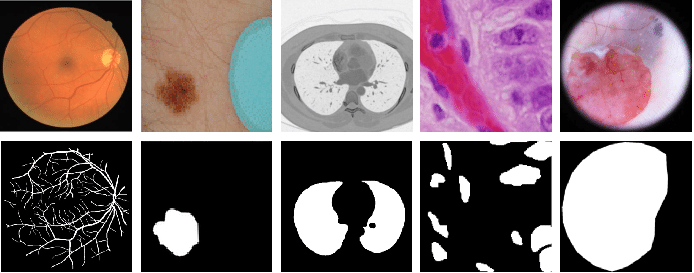
\includegraphics[width=1\linewidth]{recursos/imagens/introduction/medical-image-segmentation.png}
    \label{intro:fig:1}

    Fonte: \cite{Asadi-Aghbolaghi2020}.
\end{figure}

Outro contexto que tem usufruído muito das segmentações é o de sistemas autônomos \cite{Kaymak2019, Liu2020, Pan2020, Teichmann2018}, dos quais se cita os de máquinas empresariais para controle de qualidade e os carros autônomos, que necessitam realizar a segmentação de pedestres, placas e sinaleiros, como nos trabalhos realizados por \cite{Lee2018, Fleyeh2004, Pan2020}, dos quais é possível observar exemplos a partir da Figura \ref{intro:fig:2}.

\begin{figure}[H]
    \centering
    \caption{Exemplos de segmentação feita por sistemas autônomos.}
    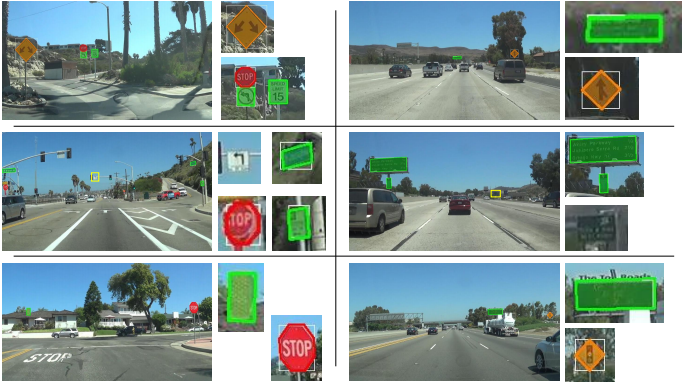
\includegraphics[width=1\linewidth]{recursos/imagens/introduction/placas.png}
    \label{intro:fig:2}

    Fonte: \cite{Lee2018}.
\end{figure}

Todavia, como citado no início deste capítulo, as segmentações não geram diretamente uma ação, mas são altamente difundidas como um processo intermediário para o reconhecimento de imagens ou detecção de objetos, como ocorre no trabalho executado por \cite{Carneiro2021}, que utiliza do método \textit{GrabCut} \cite{rother2004grabcut}, um método de segmentação baseado em grafos (que também são comuns no contexto de segmentação, como apresentado por \cite{Yi2012}) para realizar a segmentação das folhas de café antes de realizar a detecção de doenças e pragas na folha do café, como demonstrado na Figura \ref{intro:fig:3}. Este tipo de abordagem para as segmentações de imagens é muito comum como forma auxiliar em relação ao fluxo completo de sistemas de visão computacional.

\begin{figure}[H]
    \centering
    \caption{Segmentação feita com \textit{GrabCut}.}
    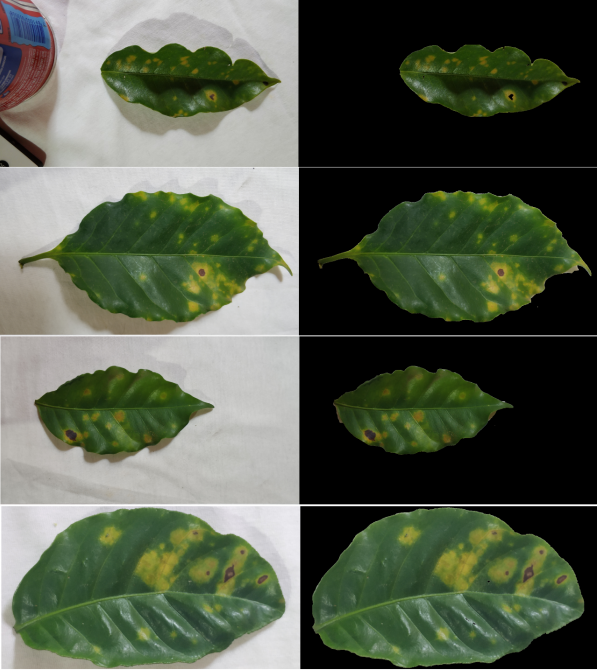
\includegraphics[height=3in]{recursos/imagens/introduction/grabcut.png}

    \label{intro:fig:3}

    Fonte: \cite{Carneiro2021}.
\end{figure}

Quanto às áreas de aplicação que viabilizam o uso das técnicas de segmentação e podem usufruir da mesma, vale citar a área odontológica, em que há uma busca em relação à exploração de todos os componentes presentes na boca dos pacientes, desde doenças (como as cáries) até a contagem e classificação de saúde dos dentes, como exemplificado na Figura \ref{intro:fig:4}. Para várias dessas atividades, o diagnóstico é acompanhado de análises de imagens clínicas, buscando evidenciar as necessidades com o uso de aparelhos \cite{Schwendicke2020}. Deste modo, como citado por \cite{Bansal2021, Nguyen2021,Schwendicke2020}, destaca-se que as soluções para esses tipos de problemas têm sido encontradas com a aplicação de inteligência artificial que aumentam o desempenho da atuação humana.

\begin{figure}[H]
    \centering
    \caption{Exemplo de segmentação na área odontológica.}
    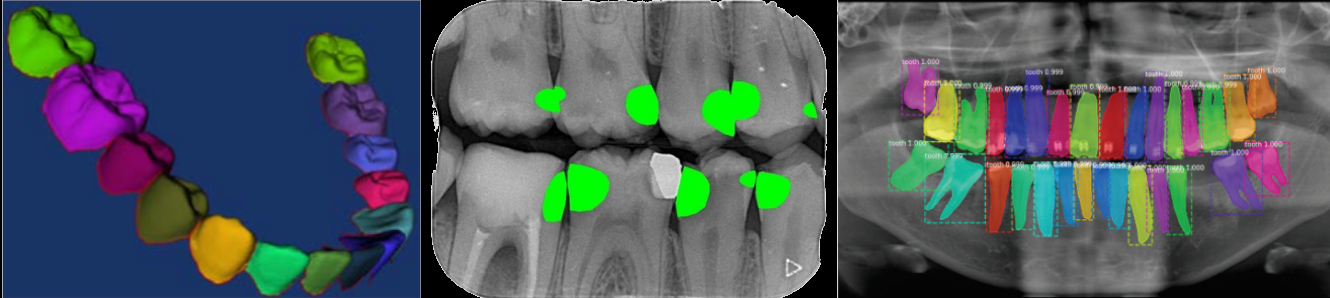
\includegraphics[width=1\linewidth]{recursos/imagens/introduction/odonto_segmentation.png}
    \label{intro:fig:4}

    Fonte: retirado e adaptado de \cite{Shuai2016,Bayrakdar2021,Gil2019}, respectivamente.
\end{figure}

Dentre as abordagens de segmentação, vale dizer que muitos algoritmos foram desenvolvidos para suprir a necessidade de segmentação, dos quais se destacam métodos artesanais (que serão trabalhados no Capitulo \ref{segment:image}), como os baseados em região ou limiar (Seção \ref{segment:region}), em bordas (Seção \ref{segment:limit}) e agrupamentos (Seção \ref{segment:group}) ou até em métodos mais complexos, devido ao progresso proporcionado pelos avanços de redes neurais, como os algoritmos baseados nessa hipótese (Seção \ref{segment:neural}).

Todavia, na medida em que algumas propostas utilizadas em inteligência artificial vêm avançando, observa-se diversos avanços nas áreas de aprendizado profundo, tendo grande destaque e evolução quanto ao âmbito de segmentação de imagens. Esses avanços ocorrem não só devido a um \textit{hardware} com mais capacidade de processamento ou uma maior quantidade de dados disponíveis, mas também por causa da criação de novos algoritmos e abordagens para resolver esses problemas \cite{Szegedy2015}.

A partir desses modelos mais modernos que utilizam como recurso o aprendizado profundo, cita-se que estes possuem capacidade de segmentar e propor classes para todos os pixels de uma imagem \cite{Minaee2021}, outros são capazes de segmentar objetos de mesma classe como instâncias diferentes, ou ainda outros que propõe fazer a unificação de ambas propostas anteriores dando um maior detalhamento das cenas, como é o caso das segmentações semânticas (Capitulo \ref{semantic:semantic}), de instâncias (Capitulo \ref{instance:instance}) e panóptica (Capitulo \ref{panoptic:panoptic}), respectivamente.

No presente projeto serão listados alguns modelos de algoritmos e \textit{frameworks} conhecidos, dos quais alguns são definidos como estado-da-arte (\textit{Mask} R-CNN e \textit{Fully Convolutional Networks}, por exemplo), de modo que estes estejam relacionados a segmentações e que seja possível encontrar vantagens, desvantagens e possibilidades de exploração em relação aos mesmos para basear novos experimentos, assim, contribuindo para a evolução científica na esfera de segmentações, principalmente das que fazem uso de aprendizado profundo.

Dentre as áreas citadas, destaca-se que na área odontológica é possível encontrar diversos desafios que podem ser otimizados com o uso de modelos de segmentações modernos - como realizado por \cite{Ghazvinian2021, Minyoung2020} - o que não é muito comum, visto que normalmente utiliza-se os métodos tradicionais \cite{Hammad2020}.  O projeto de segmentação vai de encontro ao auxilio de profissionais da área resultando em uma descrição da boca do paciente, logo colaborando para o diagnóstico \cite{Ghazvinian2021}. Sendo assim, como proposta principal desse trabalho tem-se a investigação de um arcabouço para segmentação panóptica de fotografias bucais baseado em aprendizado profundo, visando obter automaticamente uma descrição detalhada (relatório dos componentes visuais) da condição bucal de pacientes, sendo este detalhamento multinível, como uma hierarquia dos componentes visuais.

Assim, espera-se que esta investigação possa contribuir para a geração futura de uma ferramenta automática para a geração detalhada de sobre as condições bucais e dentais de pacientes. Além de poder contribuir com os profissionais dentistas, isso pode contribuir como uma ferramenta de auxílio inicial ao diagnóstico e triagem, algo importante para locais do planeta que possui recursos e acessos escassos para o tratamento odontológico.

Por fim, nos capítulos seguintes, assuntos relacionados à apresentação de conceitos de redes neurais profundas e redes neurais convolucionais serão tratadas no Capítulo \ref{deep:deep}. Após, será discorrido sobre as técnicas que tradicionalmente são utilizadas para atividades de segmentação no Capítulo \ref{segment:image}, acompanhada de segmentações que são fruto do advento das redes convolucionais e aprendizado profundo, tratando da segmentação semântica (Capítulo \ref{semantic:semantic}), de instâncias (Capítulo \ref{instance:instance}) e panóptica (Capítulo \ref{panoptic:panoptic}), para quê, finalmente sejam apresentados os detalhes da metodologia proposta nesse trabalho de forma clara no Capítulo \ref{proposal:proposal}.  Finalmente, o Capítulo \ref{final:final} apresenta algumas considerações finais do trabalho.